\documentclass{ctexart}
\usepackage{ctex}
\usepackage{geometry}
\usepackage{enumitem}
\usepackage{indentfirst}
\usepackage{color}
\usepackage{fancyhdr}
\usepackage{amsmath}
\usepackage{graphicx}

% 设置纸张和页边距——A4
\geometry{papersize={21cm,29.7cm}}
\geometry{left=3.18cm,right=3.18cm,top=2.54cm,bottom=2.54cm}

% 一级标题靠左
\CTEXsetup[format={\Large\bfseries}]{section}

% 去除页眉
\pagestyle{plain}

% 开始文档内容
\begin{document}

\title{信号与系统课程笔记:Lecture 1}
\author{授课教师:秦雨潇 \\
        笔记记录:李梦薇}
\date{2023 年 09 月 08 日(第一周,周三)}
\maketitle

\section{信号与系统是第几次关键的“技术革新”?}
\begin{enumerate}[itemindent=2em,label=(\arabic*)]
    \item 第一次:方程。例如:鸡兔同笼的问题,建立方程组解决。
    \item 第二次:微积分。离散到连续。
    \item 第三次:从三维到另一个维度。信号与系统。
\end{enumerate}

\section{什么是信号?}
信号是\textbf{带有信息}(如语言、音乐、图像、数据等)的随时间(和空间)变化的物理量或物理现象,其图像称为信号的波形。\par
信号具有相对性。\par
Signal is a function that convays information about a phenomenon. \par
Any Quantity that can vary over space or time can be used as a signal to share messages between observers.

\section{什么是系统?}
系统是由若干相互关联的单元组合而成的具有某种功能以用来达到某些特定目的的有机整体。\par
系统是信号的载体。例如:手机、人······\par
我们需要什么样的系统?\par
% 插入图像
\begin{figure}[htbp]
    \centering
    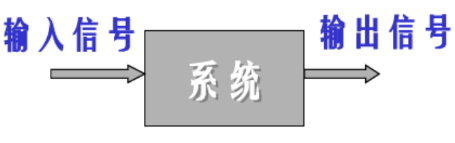
\includegraphics[width=6cm,height=2cm]{系统.png}
    \caption{系统}
\end{figure}

\section{我们希望研究什么?}
\subsection{信号的性质}
\begin{enumerate}[itemindent=2em,label=(\arabic*)]
    \item 如何识别信息?
    \item 如何处理信号?
\end{enumerate}
\subsection{系统的性质}
如何制造系统?
\begin{enumerate}[itemindent=2em,label=(\arabic*)]
    \item 时不变(Time Invariant,TI)
    \item 线性(Linear,L)
\end{enumerate}

\section{学习思路}
下面以乘法为例来介绍学习思路。\par
\begin{enumerate}[itemindent=2em,label=(\arabic*)]
    \item 思考:为什么乘法口诀表只有 $9\times9$ ?
    \item 设定 $\otimes$ 表示信号与系统中的运算,类似于乘法进行处理,那么:
          \begin{equation}
            \begin{aligned}
                12\otimes9 &= (10+2)\otimes9 \\
                &= 10\otimes9+2\otimes9 \\
                &= (1\otimes9)\times10+2\otimes9
            \end{aligned}
          \end{equation}
    \item 将超过“$9\otimes9$”的算数转换为乘法口诀表来计算,归纳为:
          \begin{equation}
            \begin{aligned}
                a\otimes{b} &= (a_1+a_2)\otimes{b} \\
                &= (c_1d_1+c_2d_2)\otimes{b} \\
                &= c_1(d_1\otimes{b})+c_2(d_2\otimes{b})
            \end{aligned}
          \end{equation}
\end{enumerate}\par
综上所述,思路为定下假设后,由简到难分解。

\section{问题}
\begin{enumerate}[itemindent=2em,label=(\arabic*)]
    \item 如何把复杂数字分解成一般数字?
    \item 一般数字怎么响应?
    \item 系统如何运转?
\end{enumerate}\par
\textbf{注意:}要理性分析!

\end{document}